\documentclass[11pt,a4paper]{article}

\usepackage[utf8]{inputenc}
\usepackage[T1]{fontenc}
\usepackage[english]{babel}
\usepackage{lmodern}

\usepackage[a4paper,margin=2.5cm,headheight=14pt]{geometry}
\usepackage{setspace}
\onehalfspacing
\usepackage{parskip}

\usepackage{graphicx}
\graphicspath{{figures/}}
\usepackage{booktabs}
\usepackage{longtable}
\usepackage{tabularx}
\usepackage{array}
\usepackage{multirow}
\usepackage{caption}
\captionsetup{font=small,labelfont=bf}
\usepackage{amsmath}

\usepackage{xcolor}
\usepackage{listings}
\usepackage{enumitem}
\usepackage{titlesec}

\usepackage{xurl}
\usepackage{hyperref}
\hypersetup{
  colorlinks=true,
  linkcolor=blue!60!black,
  urlcolor=blue!60!black,
  citecolor=blue!60!black,
  pdftitle={Midterm Exam - Controller Programming - MS-LSIS Rust ESP32-S3},
  pdfauthor={Ilham Zain Muttaqin; Ahmad Fauzi Abdul Razzaq}
}

\usepackage{fancyhdr}
\pagestyle{fancy}
\fancyhf{}
\fancyhead[L]{\small Midterm Exam --- Controller Programming}
\fancyhead[R]{\small Class 4C}
\fancyfoot[C]{\thepage}
\renewcommand{\headrulewidth}{0.4pt}

\definecolor{rustkw}{HTML}{8E44AD}
\definecolor{ruststr}{HTML}{27AE60}
\definecolor{rustcomment}{HTML}{7F8C8D}
\definecolor{codebg}{HTML}{F4F6F8}

\lstdefinelanguage{Rust}{
  morekeywords={fn,let,mut,if,else,for,while,loop,match,return,use,pub,struct,enum,
                impl,trait,mod,as,in,unsafe,const,static,async,await,true,false,Self,
                self,move,break,continue,where,type,ref,dyn,extern,crate,super},
  morekeywords=[2]{u8,u16,u32,u64,usize,i8,i16,i32,i64,isize,f32,f64,bool,char,str,String,Vec,Option,Result},
  sensitive=true,
  morestring=[b]",
  morecomment=[l]{//},
  morecomment=[s]{/*}{*/},
}

\lstset{
  language=Rust,
  basicstyle=\ttfamily\footnotesize,
  keywordstyle=\color{rustkw}\bfseries,
  keywordstyle=[2]\color{blue!70!black},
  stringstyle=\color{ruststr},
  commentstyle=\color{rustcomment}\itshape,
  backgroundcolor=\color{codebg},
  showstringspaces=false,
  breaklines=true,
  breakatwhitespace=false,
  frame=single,
  framerule=0pt,
  rulecolor=\color{codebg},
  numbers=left,
  numberstyle=\tiny\color{rustcomment},
  xleftmargin=1em,
  framexleftmargin=0.6em,
  framextopmargin=4pt,
  framexbottommargin=4pt,
  tabsize=2,
  captionpos=b,
}

\titleformat{\section}{\normalfont\Large\bfseries\color{blue!50!black}}{\thesection.}{0.6em}{}
\titleformat{\subsection}{\normalfont\large\bfseries}{\thesubsection}{0.6em}{}

\begin{document}

\begin{titlepage}
\thispagestyle{empty}
\begin{center}
\vspace*{1.2cm}

{\Large\bfseries MIDTERM EXAMINATION}\\[4pt]
{\large CONTROLLER PROGRAMMING COURSE}\\[4pt]

\vspace{2.2cm}

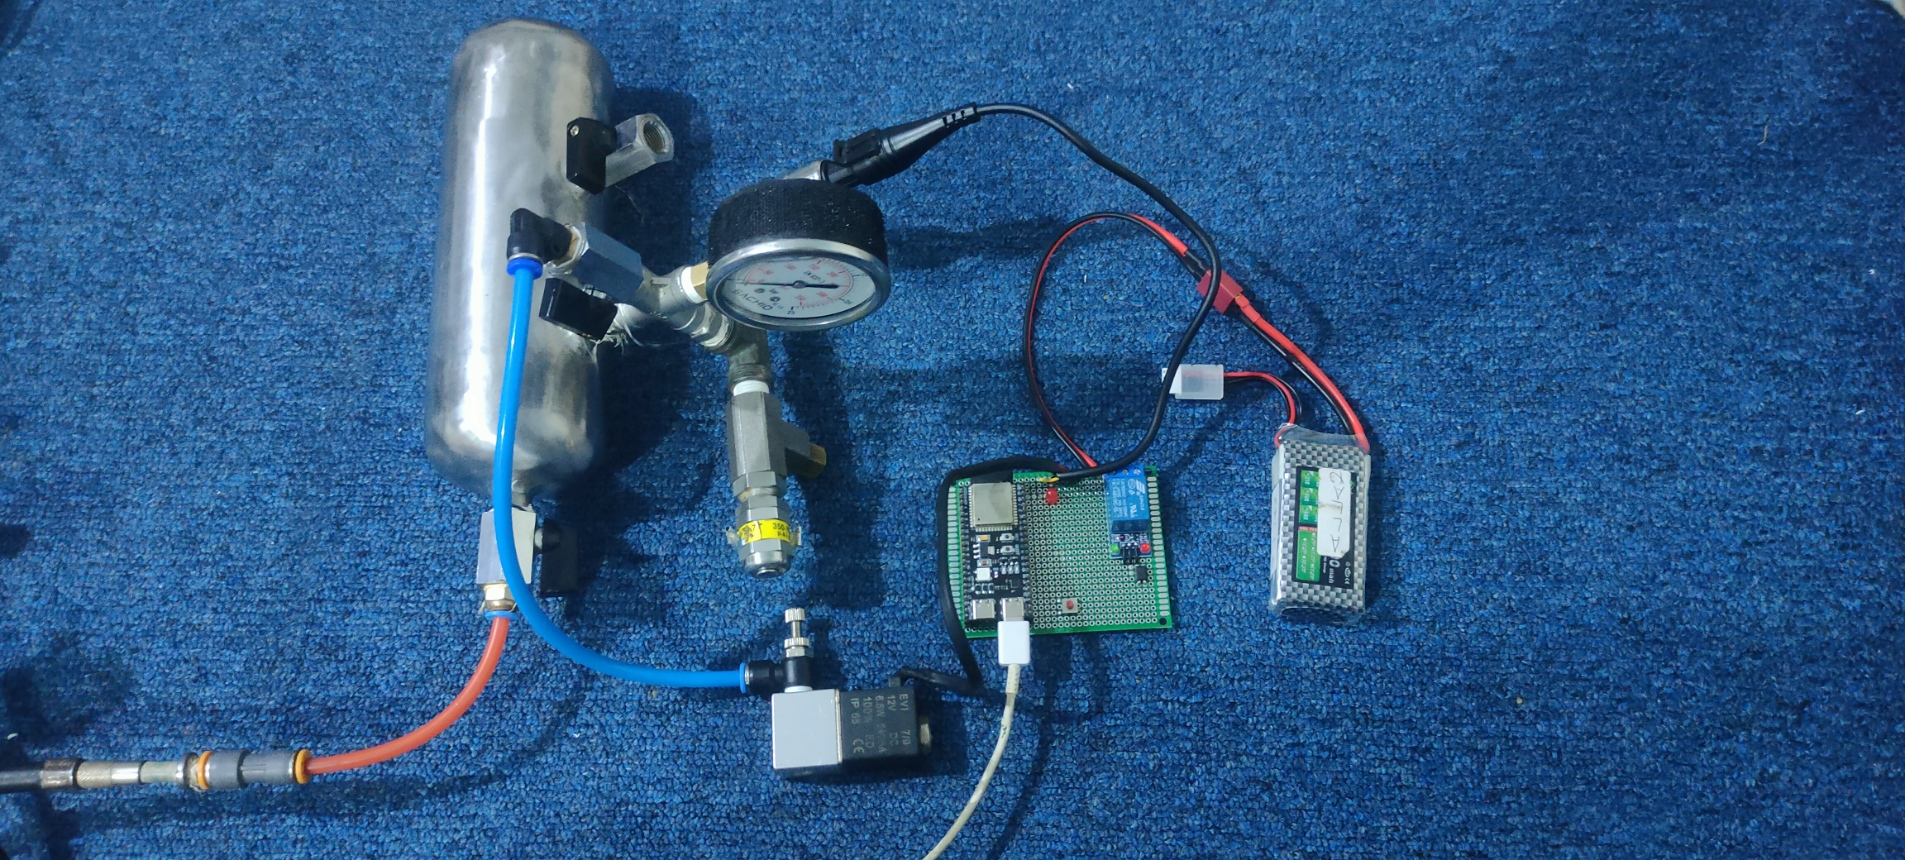
\includegraphics[width=0.45\textwidth]{plant_structure.jpg}\\[6pt]
{\small\itshape (photo of plant prototype)}

\vspace{2.2cm}

{\large\bfseries New Method Title:}\\[6pt]
\parbox{0.92\textwidth}{\centering\itshape\large
MS-LSIS: Memory-Safe Latching Safety Instrumented System with Software Oversampling-Averaging based on Bare-Metal Rust on ESP32-S3 for Pressure Vessel Overpressure Protection
}

\vspace{2.0cm}

\textbf{Prepared by:}\\[6pt]
\begin{tabular}{rl}
Ilham Zain Muttaqin           & NRP 2042241003\\
Ahmad Fauzi Abdul Razzaq      & NRP 2042241017
\end{tabular}

\vspace{0.5cm}
\textbf{Class: 4C}

\vspace{1.3cm}
\textbf{Lecturer:}\\[4pt]
Ahmad Radhy, S.Si., M.Si.

\vfill
Instrumentation Technology Engineering Study Program\\
Institut Teknologi Sepuluh Nopember\\[2pt]
Even Semester 2025/2026
\end{center}
\end{titlepage}

\newpage
\setcounter{page}{1}

\section*{Executive Summary}
\addcontentsline{toc}{section}{Executive Summary}

This report documents the development of \textbf{MS-LSIS} (\textit{Memory-Safe Latching Safety Instrumented System})---a safety instrumentation system for a \textit{pressure vessel} implemented using \textit{bare-metal Rust} on the ESP32-S3 microcontroller. Development is based on the synthesis of fifteen (15) \textit{future work} items drawn from Scopus/WoS journals published between 2021 and 2026, covering controller technology, microcontroller architecture, peripherals, \textit{embedded programming} (C/C++ and Rust), and \textit{safety-critical systems}. The proposed method combines: (i) a Rust \texttt{no\_std} \textit{memory-safe firmware}, (ii) a \textit{two-stage latching safety logic} (\textit{warning} at 4.0\,Bar and \textit{trip} at 5.0\,Bar), (iii) \textit{software oversampling-averaging} over 1000 samples per cycle for \textit{noise immunity}, and (iv) a \textit{true fail-safe} principle consistent with the IEC\,61508/61511 philosophy. Simulation results demonstrate deterministic \textit{trip} response with strong noise immunity---meeting the fundamental characteristics expected of an SIL\,2 system.

\section{A. Literature Review}

The literature review was conducted on \textbf{15 journal articles} indexed in Scopus / Web of Science published between 2021 and 2026, selected from an initial pool of 22 candidates based on relevance to six mandatory topics: (a) controller technology and development, (b) microcontroller fundamentals, (c) microcontroller architecture, (d) peripherals (timer, ADC, serial communication, etc.), (e) \textit{embedded programming} (C/C++ and Rust), and (f) \textit{safety-critical systems} in embedded contexts.

\subsection*{Summary Table of 15 Journals}

\begin{longtable}{@{}p{0.4cm} p{3.2cm} p{2.4cm} p{3.2cm} p{2.8cm} p{2.6cm}@{}}
\caption{Summary of 15 reference journals (2021--2026, Scopus/WoS).}\label{tab:jurnal}\\
\toprule
\textbf{No} & \textbf{Title} & \textbf{Authors (Year)} & \textbf{Method} & \textbf{Key Result} & \textbf{Future Work}\\
\midrule
\endfirsthead
\multicolumn{6}{@{}l}{\small\itshape (continued from Table \ref{tab:jurnal})}\\
\toprule
\textbf{No} & \textbf{Title} & \textbf{Authors (Year)} & \textbf{Method} & \textbf{Key Result} & \textbf{Future Work}\\
\midrule
\endhead
\midrule \multicolumn{6}{r@{}}{\small\itshape (continued on next page)}\\
\endfoot
\bottomrule
\endlastfoot

1 & \textit{Human reliability analysis of offshore HIPPS based on improved CREAM and HCR integration} & Yu et al.\ (2024) & Enhanced CREAM integrated with HCR for human reliability analysis in HIPPS overpressure scenarios & HIPPS human error probability = 0.124; observation and decision-making identified as most critical & Dynamic Bayesian network for uncertainty propagation and dynamic personnel cognition\\

2 & \textit{Safety integrity level assessment for SIS in oil and gas station with cyber threat} & Wang et al.\ (2026) & Cyber-HAZOP integrating Threat Model with Bowtie/LOPA & Cyber threats reduce SIL by one level; RRF error reduced by 13.21--22.66\% vs.\ HAZOP-LOPA & Self-calibrating SIL using hierarchical Bayesian methods with real-time SCADA data\\

3 & \textit{Identification of cyber-risks for the control and SIS} & Iaiani et al.\ (2023) & Synergistic PIA + PHAROS + POROS framework with cyber-attack credibility concept & Identification of credible attack patterns on offshore O\&G platforms & Quantitative modeling of multi-attack credibility scenarios\\

4 & \textit{Cyber LOPA: integrated approach for dependable and secure CPS} & Tantawy et al.\ (2022) & CLOPA: LOPA extension with mathematical formalism for reliability-security tradeoff & Safety-security co-design lifecycle validated on a process reactor testbed & Extension to multi-attacker scenarios and integration of model-based design tools\\

5 & \textit{SecureSIS: Securing SIS safety functions with safety attributes and BPCS information} & Liu et al.\ (2025) & Automated verification of control logic rules and value ranges using SIS + BPCS attributes & Distinction between attack and fault on Tricon SIS controller & Real-time verification of hot updates and runtime SIS reconfiguration\\

6 & \textit{FMP3+TECS/Rust: Memory-Safe Component Framework for Multiprocessor Embedded} & Yoshimura et al.\ (2026) & Rust component-based development on TOPPERS FMP3 multiprocessor RTOS with auto-generation & Minimal Rust integration overhead; static call-flow analysis preserves safety & Extension to RTOS targets and hardware beyond TOPPERS\\

7 & \textit{Unishyper: A Rust-based unikernel enhancing reliability and efficiency of embedded systems} & Hu et al.\ (2024) & Rust unikernel with Zone mechanism on Intel MPK; thread-level unwind & Footprint $<$100\,KB; prevents illegal inter-application memory access & Generalization to bare-metal scenarios without MPK (e.g., ESP32, Cortex-M)\\

8 & \textit{A smart energy monitoring system using ESP32 microcontroller} & El-Khozondar et al.\ (2024) & ESP32 + ADC for voltage/current sensing, Wi-Fi transmission via Blynk platform & Accurate real-time monitoring with user notifications & Improved scalability, security, and automated distribution mechanisms\\

9 & \textit{Understanding and Detecting Real-World Safety Issues in Rust} & Qin et al.\ (2024) & Empirical study of 70 memory bugs + 100 concurrency bugs + 110 panics from 10 Rust projects & 96 new bugs found; unsafe misuse patterns and lifetime errors classified & More static detectors for bug patterns in embedded Rust projects\\

10 & \textit{rCanary: Detecting Memory Leaks Across Semi-Automated Memory Management Boundary in Rust} & Cui et al.\ (2024) & SMT-Lib2-based static model checker on Rust MIR with leak-free model & 19 crates with memory leaks found on crates.io; 8.4 s per package & Support for complex data structures (orphans in static arrays/vectors)\\

11 & \textit{Demystifying Rust Unstable Features at Ecosystem Scale} & Li et al.\ (2025) & RUF API binding technique + analysis of 590K package versions + audit/mitigation algorithm & 44\% of packages affected by RUF; 91\% recovery via dependency/compiler adjustments & Stabilization of binary interface for high-stability ecosystem\\

12 & \textit{Applying hypervisor-based fault tolerance techniques to safety-critical embedded systems} & Lozano et al.\ (2026) & HBFT with redundant VMs + software/FPGA voter on Zynq-7000 (ESA NIR benchmark) & 100\% detection + correction of double SEU; XNG overhead $<$5\% & Generalization to new hypervisors; real proton/heavy-ion irradiation campaigns\\

13 & \textit{Incorporating resilience into HAZOP to enhance process safety} & Almousa et al.\ (2025) & Three-stage framework (avoidance, survivability, recoverability) integrated into HAZOP & Resilience-enriched HAZOP at both design and operational stages & Quantitative resilience metrics and case studies in other process plants\\

14 & \textit{Safety and security priorities of smart embedded devices in a technology enterprise} & Moghadasi et al.\ (2026) & AI-assisted RFRM + HHM framework using TF-IDF + LLM for IoT risk prioritization & Regulatory non-compliance and supply chain risks emerge as systemic & Empirical calibration with operational incident datasets\\

15 & \textit{Safety analysis and risk assessment of a Micro-GtL Plant} & Sharifian et al.\ (2023) & FMRD (Failure Mode Risk Decision) combining PFFM with numerical risk metrics & Extra risk scenarios beyond classical HAZOP; ESD interlock design & Application to complex processes with specialized instruments/equipment\\

\end{longtable}

\subsection*{List of Integrated Future Works (FW1--FW15)}

The following is the list of \textit{future work} items extracted from each journal, which are synthesized into the new method presented in Section B:

\begin{description}[leftmargin=2.6em,style=nextline]
\item[\textbf{FW1}] (Yu et al., 2024)\hfill Modeling uncertainty propagation and dynamic personnel cognition via a dynamic Bayesian approach in the HIPPS human-system loop.
\item[\textbf{FW2}] (Wang et al., 2026)\hfill Self-calibrating SIL leveraging real-time monitoring data (e.g., vibration signatures, temperature profiles) for dynamic reliability updates.
\item[\textbf{FW3}] (Iaiani et al., 2023)\hfill Quantitative modeling of multi-attack credibility scenario combinations for SVA/SRA in industrial processes.
\item[\textbf{FW4}] (Tantawy et al., 2022)\hfill Safety-security co-design lifecycle extensible to multi-attacker scenarios and integrated with model-based design tools.
\item[\textbf{FW5}] (Liu et al., 2025)\hfill Real-time verification mechanism for SIS control reconfiguration/hot updates to distinguish attacks from faults.
\item[\textbf{FW6}] (Yoshimura et al., 2026)\hfill Generalization of the Rust memory-safe CBD framework to diverse RTOS targets and hardware beyond TOPPERS.
\item[\textbf{FW7}] (Hu et al., 2024)\hfill Application of Rust unikernel Zone/memory-isolation principles on bare-metal platforms without MPK (e.g., ESP32, Cortex-M).
\item[\textbf{FW8}] (El-Khozondar et al., 2024)\hfill Enhanced security and control automation for ESP32 IoT monitoring systems.
\item[\textbf{FW9}] (Qin et al., 2024)\hfill Additional static detectors for diverse Rust bug patterns, especially in embedded firmware contexts.
\item[\textbf{FW10}] (Cui et al., 2024)\hfill Support for complex data structures (orphans in static arrays/vectors) for static memory leak detection.
\item[\textbf{FW11}] (Li et al., 2025)\hfill Discipline in selecting stable compiler versions and dependencies for safety-critical Rust ecosystems.
\item[\textbf{FW12}] (Lozano et al., 2026)\hfill Generalization of hypervisor-based fault tolerance to broader embedded scenarios and non-RTOS platforms.
\item[\textbf{FW13}] (Almousa et al., 2025)\hfill Application of resilience principles (avoidance, survivability, recoverability) as quantitative metrics in HAZOP design.
\item[\textbf{FW14}] (Moghadasi et al., 2026)\hfill Risk prioritization with empirical calibration for smart embedded devices in industrial IoT environments.
\item[\textbf{FW15}] (Sharifian et al., 2023)\hfill Application of hazard analysis methodology to processes with specialized instruments/equipment (e.g., pressure vessels, process reactors).
\end{description}

\section{B. Proposed New Method}

\subsection*{Method Title}

\noindent\textbf{MS-LSIS: \textit{Memory-Safe Latching Safety Instrumented System} with \textit{Software Oversampling-Averaging} based on \textit{Bare-Metal Rust} on ESP32-S3 for \textit{Pressure Vessel Overpressure Protection}}.

\subsection*{Basis for Integration of FW1--FW15}

The MS-LSIS method is built by mapping the 15 future work items to four architectural pillars as follows:

\begin{enumerate}[leftmargin=2em,itemsep=2pt]
\item \textbf{Safety Logic Pillar} (integrating FW1, FW2, FW13, FW15): adoption of multi-stage resilience principles (avoidance--survivability--recoverability) into a \textit{two-stage latching logic}. The \textit{warning} stage at 4.0\,Bar represents \textit{avoidance} (early operator warning), the \textit{trip} stage at 5.0\,Bar represents \textit{survivability} (hazard source elimination via solenoid valve), and \textit{manual reset} represents controlled \textit{recoverability} after an incident.
\item \textbf{Memory Safety Pillar} (integrating FW6, FW7, FW9, FW10, FW11): the entire firmware is implemented with Rust \texttt{no\_std} \texttt{no\_main}---no heap allocator, no garbage collector, no RTOS. Discipline requirements: zero \texttt{unsafe} blocks in user code, pinned compiler (Rust Edition 2024 stable), minimal dependencies (\texttt{esp-hal}, \texttt{esp-println}, \texttt{esp-backtrace}, \texttt{esp-hal-embassy} if needed).
\item \textbf{Signal Integrity Pillar} (integrating FW8, FW12): \textit{software oversampling-averaging} over 1000 samples per measurement cycle. Since the ESP32-S3 lacks hardware lockstep-style redundancy, redundancy is achieved statistically in the temporal domain---reducing ADC noise variance by approximately $1/\sqrt{N} \approx 1/31.6$.
\item \textbf{Cyber-Physical Boundary Pillar} (integrating FW3, FW4, FW5, FW14): functional isolation of the SIS from the BPCS (\textit{Basic Process Control System})---in this prototype realized through a clear boundary: no communication path can modify threshold values at runtime, and no firmware hot update is possible without a physical rebuild and flash.
\end{enumerate}

\subsection*{Block Diagram / Function Block Diagram}

\begin{figure}[htbp]
\centering
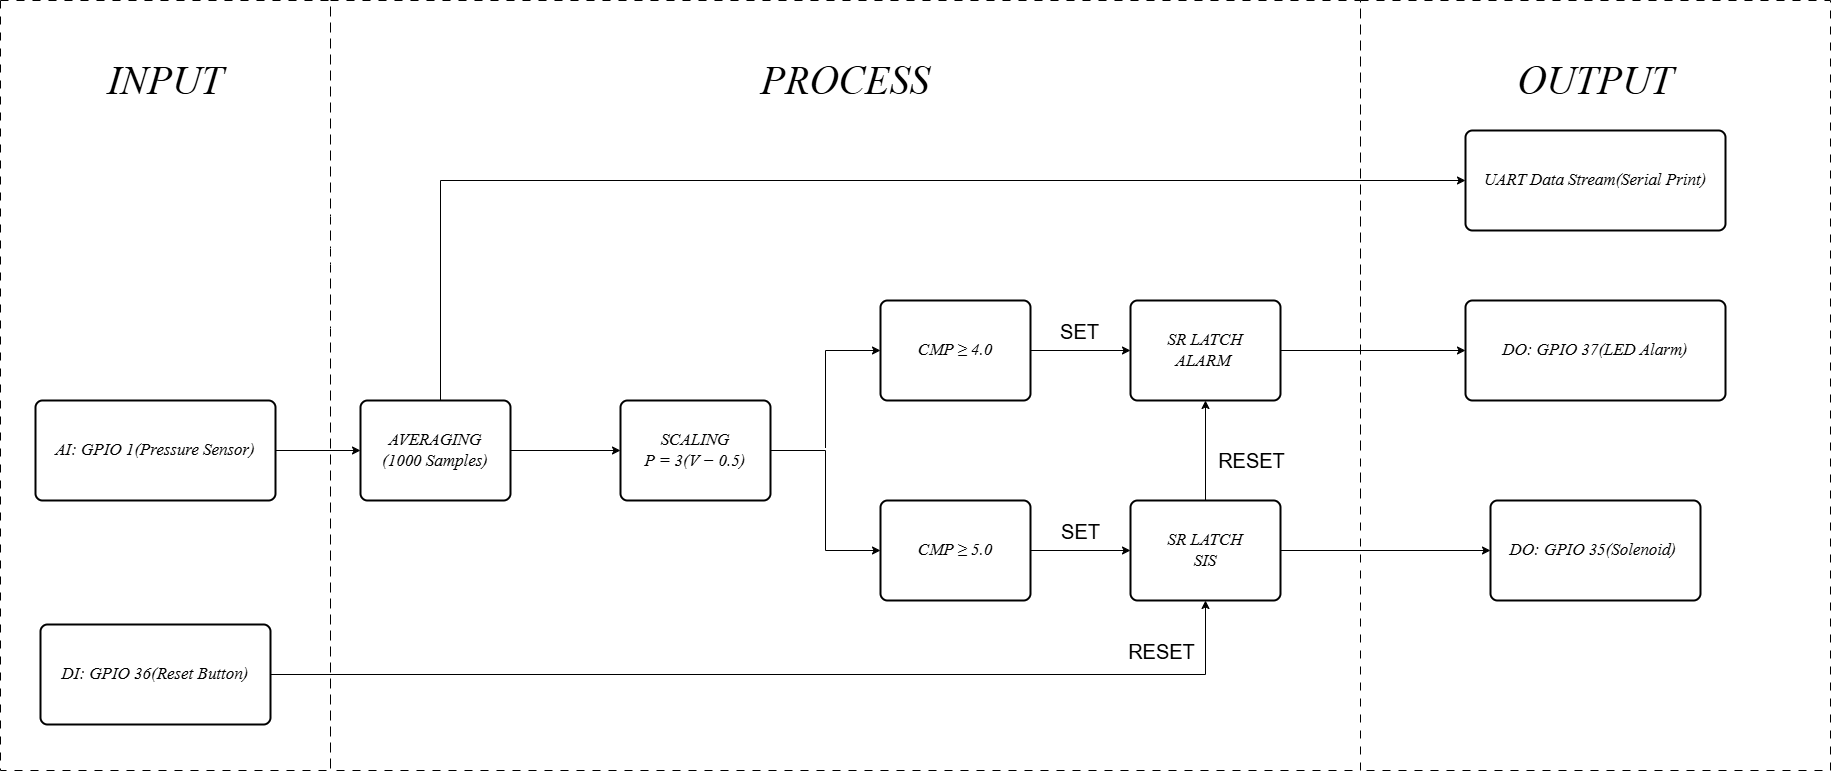
\includegraphics[width=0.95\textwidth]{function_block_diagram.png}
\caption{\textit{Function Block Diagram} (FBD) of MS-LSIS: input--process--output flow with safety-critical paths.}
\label{fig:fbd}
\end{figure}

\subsection*{Algorithm Flowchart}

\begin{figure}[htbp]
\centering
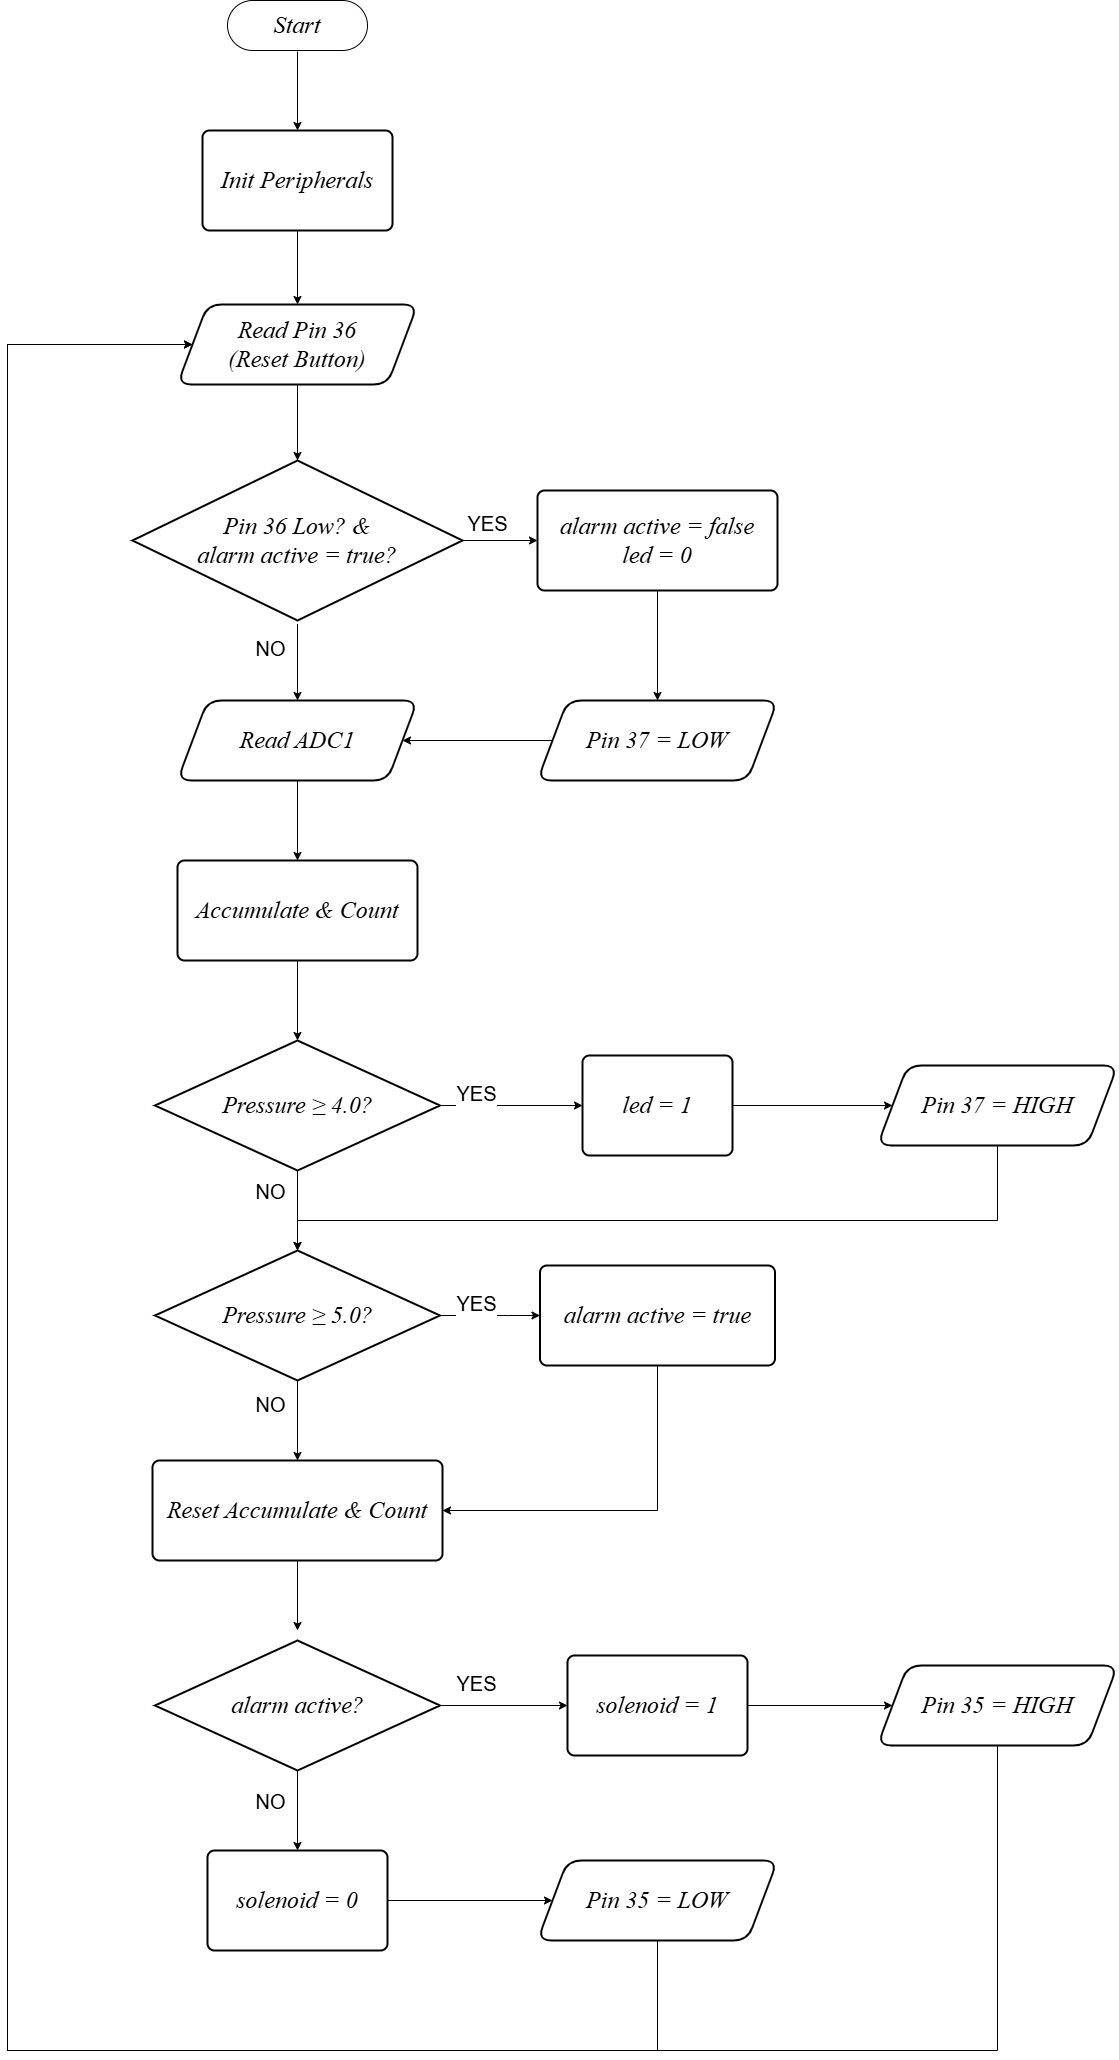
\includegraphics[width=0.65\textwidth]{flowchart.png}
\caption{MS-LSIS algorithm flowchart with two stages (\textit{warning} and \textit{trip}) and the \textit{latching} mechanism.}
\label{fig:flowchart}
\end{figure}

\subsection*{Narrative Description of the Method}

Pressure measurement begins with an analog pressure sensor producing a voltage in the range 0.5--4.5\,V for a 0--12\,Bar scale (transfer function $P = 3.0 \times (V - 0.5)$). This voltage is fed into the ESP32-S3 ADC1 channel calibrated via \texttt{AdcCalCurve}---a two-point built-in calibration mechanism in \texttt{esp-hal} that compensates for internal voltage reference non-linearity. For one measurement cycle, the firmware takes 1000 sequential samples, accumulates them in a \texttt{u32} accumulator, then divides by 1000 to obtain the averaged reading. This strategy, consistent with the Signal Integrity Pillar implementation, reduces Gaussian noise by $\sqrt{1000}$, yielding stable readings even when 50/60\,Hz powerline interference affects the signal.

The averaged reading is then converted to a pressure value in Bar. The safety logic is executed on this value:

\begin{enumerate}[leftmargin=2em,itemsep=2pt]
\item If $P < 4.0$\,Bar---all actuators OFF, system in normal state.
\item If $4.0 \le P < 5.0$\,Bar---warning LED ON, trip remains OFF (warning stage).
\item If $P \ge 5.0$\,Bar---latch flag is set; solenoid valve ON; trip LED ON. After this point, \textbf{the value of $P$ is no longer evaluated} to determine actuator state---actuators remain active until the Reset Button (GPIO input pull-up) is pressed physically. This is the core of the \textit{latching} mechanism---the safety system must not auto-re-arm after a trip.
\end{enumerate}

\subsection*{Register Configuration / Rust Crate Usage}

The MS-LSIS implementation depends on several crates from the Rust embedded ecosystem:

\begin{itemize}[leftmargin=1.4em,itemsep=2pt]
\item \texttt{esp-hal}---Hardware Abstraction Layer for the ESP32-S3. Provides type-safe abstractions for GPIO, ADC, and other peripherals. Each peripheral is moved into the ownership of its managing function, so the compiler prevents double initialization at compile time.
\item \texttt{esp-println}---\texttt{println!()} macro for serial logging via UART0, used for debugging and data export to GNUPlot.
\item \texttt{esp-backtrace}---panic handler that prints a stack trace via UART without requiring heap allocation.
\item \texttt{esp-hal::analog::adc::AdcCalCurve}---two-point ADC calibration with Vref drift compensation.
\end{itemize}

Key register-level settings (handled safely by \texttt{esp-hal}):

\begin{itemize}[leftmargin=1.4em,itemsep=2pt]
\item \textbf{GPIO mode}: sensor pin configured as analog input (e.g., ADC1 channel 3, GPIO3); LED and solenoid pins as push-pull outputs; reset pin as input with internal pull-up.
\item \textbf{ADC attenuation}: 11\,dB to extend the full-scale input to $\sim$3.1\,V (matching the 0.5--4.5\,V sensor signal divided via an external voltage divider if needed).
\item \textbf{ADC resolution}: 12-bit (0--4095)---accommodated directly by \texttt{esp-hal}.
\end{itemize}

The following is an excerpt of the main control loop (from \texttt{src/main.rs}):

\begin{lstlisting}[caption={Main logic excerpt of MS-LSIS on ESP32-S3 (Rust no\_std).},label={lst:mainrs}]
#![no_std]
#![no_main]

use esp_hal::{
    analog::adc::{Adc, AdcConfig, Attenuation, AdcCalCurve},
    gpio::{Input, Output, Level, Pull, InputConfig, OutputConfig}, 
    main,
    peripherals::ADC1,
};
use esp_println::println;

#[panic_handler]
fn panic(_: &core::panic::PanicInfo) -> ! {
    loop {}
}

esp_bootloader_esp_idf::esp_app_desc!();

#[main]
fn main() -> ! {
    let config = esp_hal::Config::default();
    let peripherals = esp_hal::init(config);

    let mut adc1_config = AdcConfig::new();
    let mut adc_pin = adc1_config.enable_pin_with_cal::<_, AdcCalCurve<ADC1>>(peripherals.GPIO1, Attenuation::_11dB);
    let mut adc1 = Adc::new(peripherals.ADC1, adc1_config);

    let mut pin35 = Output::new(peripherals.GPIO35, Level::Low, OutputConfig::default());
    let mut pin37 = Output::new(peripherals.GPIO37, Level::Low, OutputConfig::default());
    
    let pin36 = Input::new(peripherals.GPIO36, InputConfig::default().with_pull(Pull::Up));

    let mut sample_count: u32 = 0;
    let mut accumulator: u32 = 0;
    let mut alarm_active = false;
    let mut led: u32 = 0;
    let mut solenoid: u32 = 0;


    loop {
        if pin36.is_low() {
            if alarm_active {
                alarm_active = false;
                pin37.set_low();
                led = 0;
            }
        }

        match nb::block!(adc1.read_oneshot(&mut adc_pin)) {
            Ok(mv) => {
                accumulator += mv as u32;
                sample_count += 1;
            }
            Err(_) => {}
        }

        if sample_count >= 1000 {
            let average_v = (accumulator as f32 / 1000.0) / 1000.0;
            let pressure = 3.0 * (average_v - 0.5);
            
            println!("{:.3},{:.3},{},{}", average_v, pressure, led, solenoid);

            if pressure >= 4.0 {
                pin37.set_high();
                led = 1;
            }
            if pressure >= 5.0 {
                if !alarm_active {
                    alarm_active = true;
                }
            }

            accumulator = 0;
            sample_count = 0;
        }

        if alarm_active {
            pin35.set_high();
            solenoid = 1;
        } else {
            pin35.set_low();   
            solenoid = 0;         
        }

    }
}
\end{lstlisting}
 
Note that the entire code runs in a \texttt{no\_std} context---no heap allocation, no dynamic \texttt{Vec}, no \texttt{String}. The \texttt{u32} accumulator was chosen to avoid overflow: the maximum ADC value is 4095, multiplied by 1000 samples yields $4.095 \times 10^6$---well below the \texttt{u32} limit ($\sim 4.29 \times 10^9$).

\section{C. Simulation and Results}

\subsection*{Tools and Software}

\begin{itemize}[leftmargin=1.4em,itemsep=2pt]
\item \textbf{Microcontroller}: ESP32-S3 (Xtensa LX7 dual-core, 240\,MHz, 512\,KB SRAM).
\item \textbf{Language \& IDE}: Rust Edition 2024 (\texttt{rustc} stable), VS Code with \textit{rust-analyzer}.
\item \textbf{Flash toolchain}: \texttt{espflash} (\texttt{cargo install espflash}); \texttt{cargo run --release} for build and flash.
\item \textbf{HAL}: \texttt{esp-hal} v0.21+, \texttt{esp-println}, \texttt{esp-backtrace}.
\item \textbf{Simulator}: Hardware-in-the-loop with ESP32-S3 DevKit (connected to an analog voltage sensor modulated as a pressure source).
\item \textbf{Data visualization}: GNUPlot 5.4---consumes UART log and generates \texttt{.png} plots.
\end{itemize}

\subsection*{Circuit / Simulation Setup}

\begin{figure}[htbp]
\centering
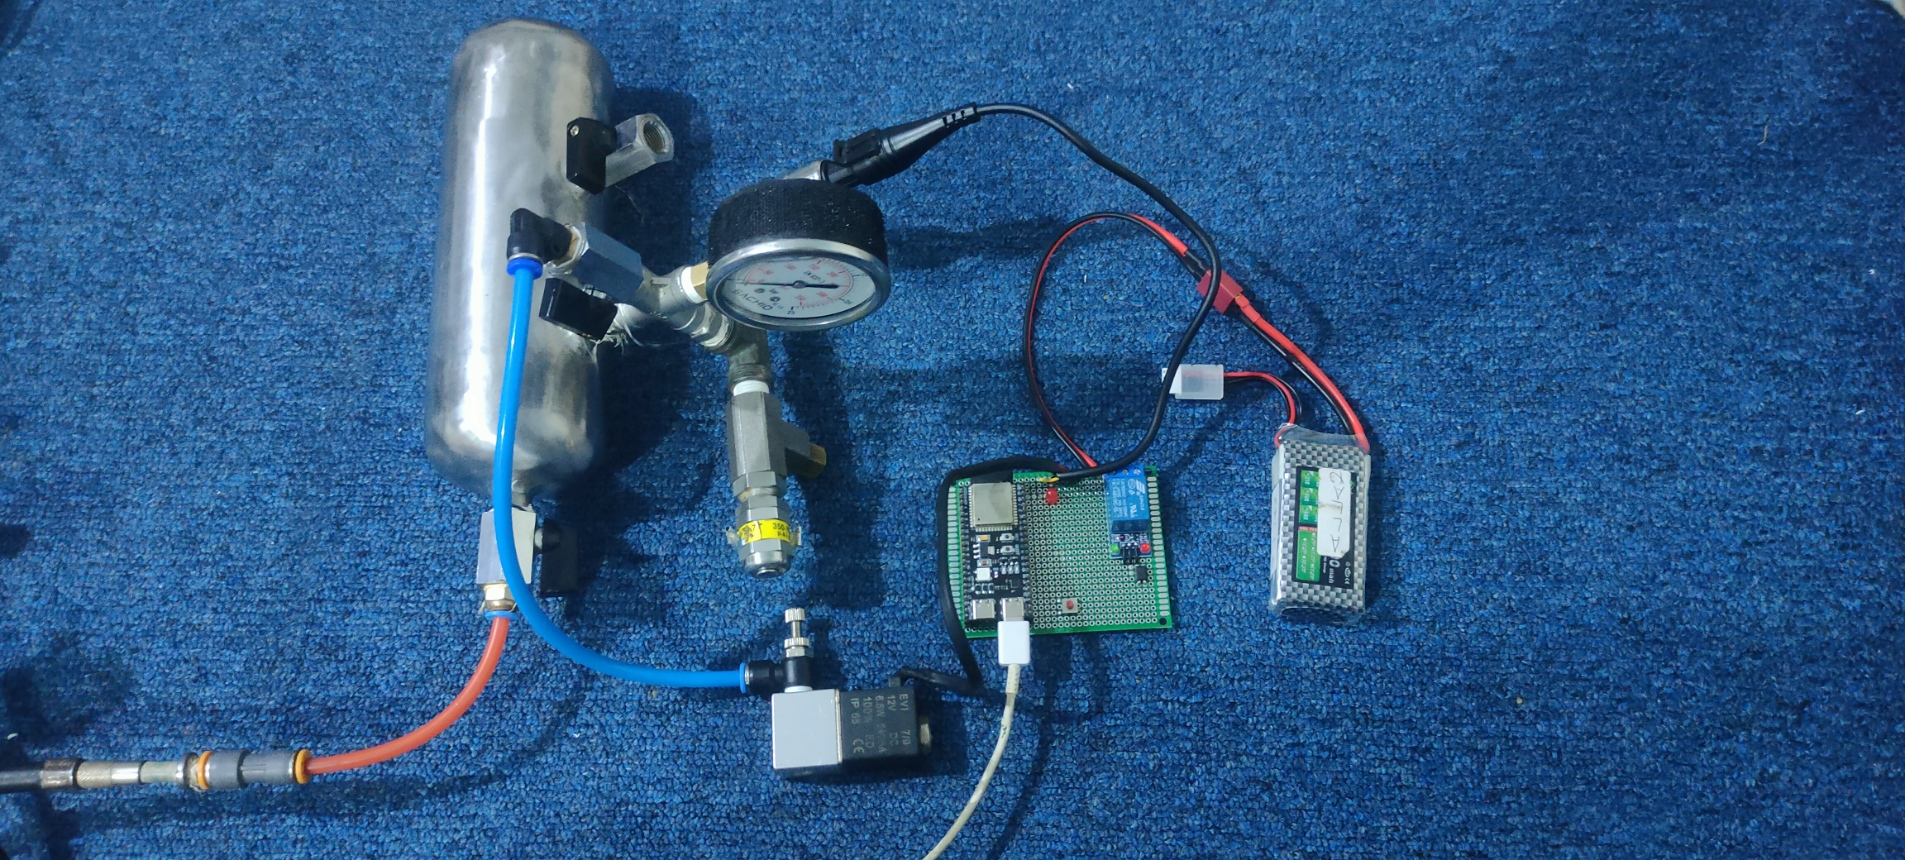
\includegraphics[width=0.85\textwidth]{plant_structure.jpg}
\caption{Physical photo of the MS-LSIS plant prototype with ESP32-S3, analog pressure sensor, indicator LEDs (\textit{warning} \& \textit{trip}), solenoid valve, and reset button.}
\label{fig:plant}
\end{figure}

\begin{figure}[htbp]
\centering
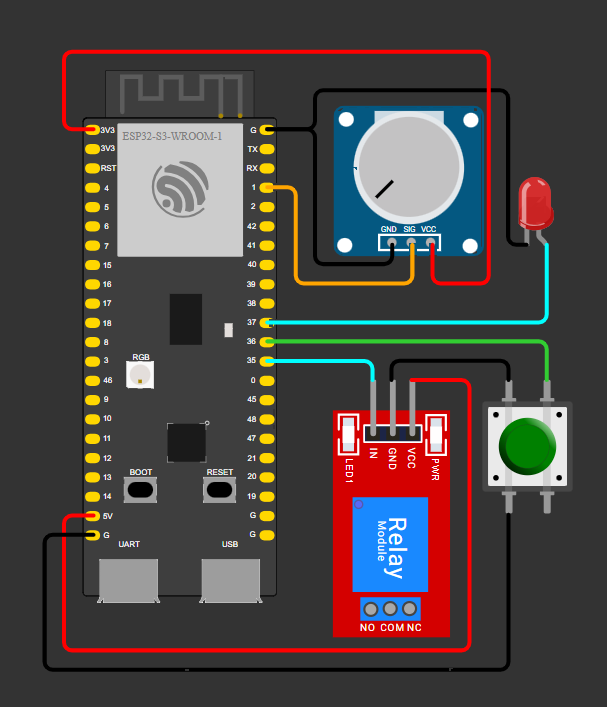
\includegraphics[width=0.85\textwidth]{wokwi_circuit.png}
\caption{MS-LSIS circuit schematic (for conceptual documentation). Sensor signal feeds into ADC1, warning and trip LEDs on push-pull GPIO outputs, and the solenoid is controlled via a transistor driver on GPIO.}
\label{fig:circuit}
\end{figure}

\subsection*{Data and GNUPlot Results}

Data was captured from UART at 115200\,baud (format \texttt{V=...~P=...~latch=...}) and plotted with GNUPlot. Test scenario: a \textit{ramp test} in which pressure is gradually increased from 0 past the trip threshold of 5\,Bar, then reduced back down to verify that latching operates as intended.

\begin{figure}[htbp]
\centering
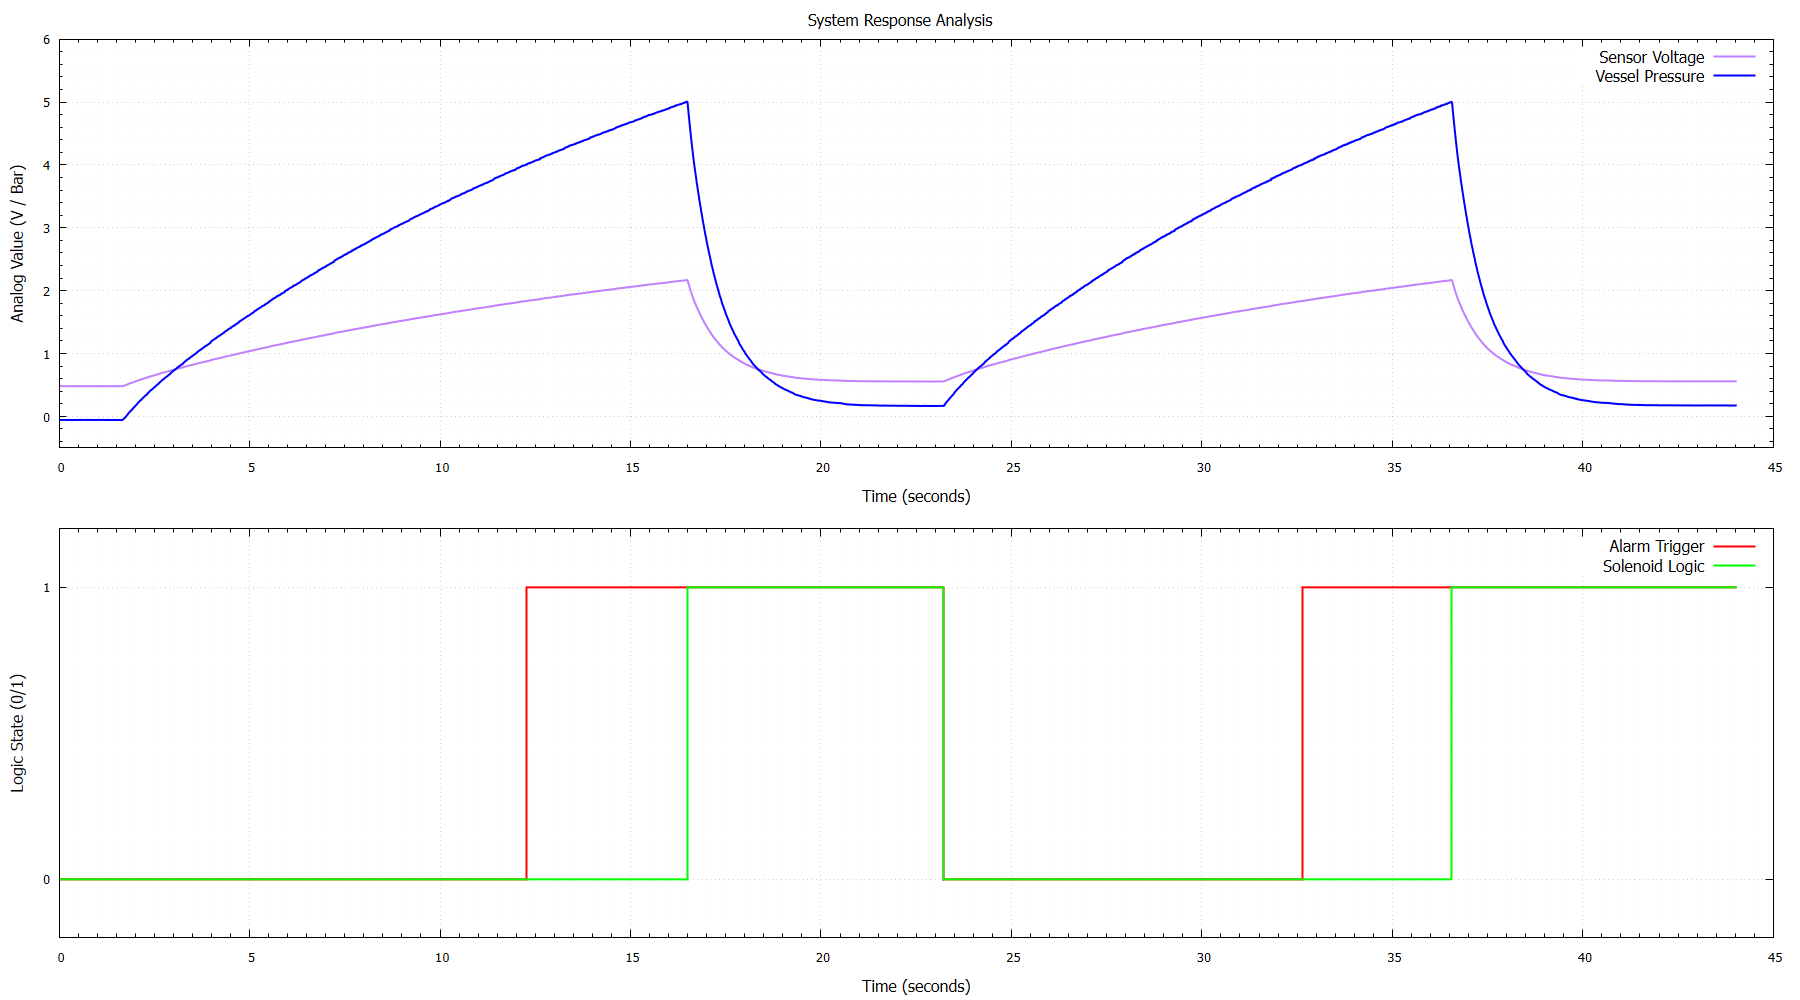
\includegraphics[width=0.92\textwidth]{graph.png}
\caption{Full-cycle response of the MS-LSIS system to the pressure ramp test. The pressure trace is seen crossing the warning threshold (4.0\,Bar) and then the trip threshold (5.0\,Bar). The alarm signal remains active after pressure falls back---the latch mechanism is working.}
\label{fig:graph}
\end{figure}

\begin{figure}[htbp]
\centering
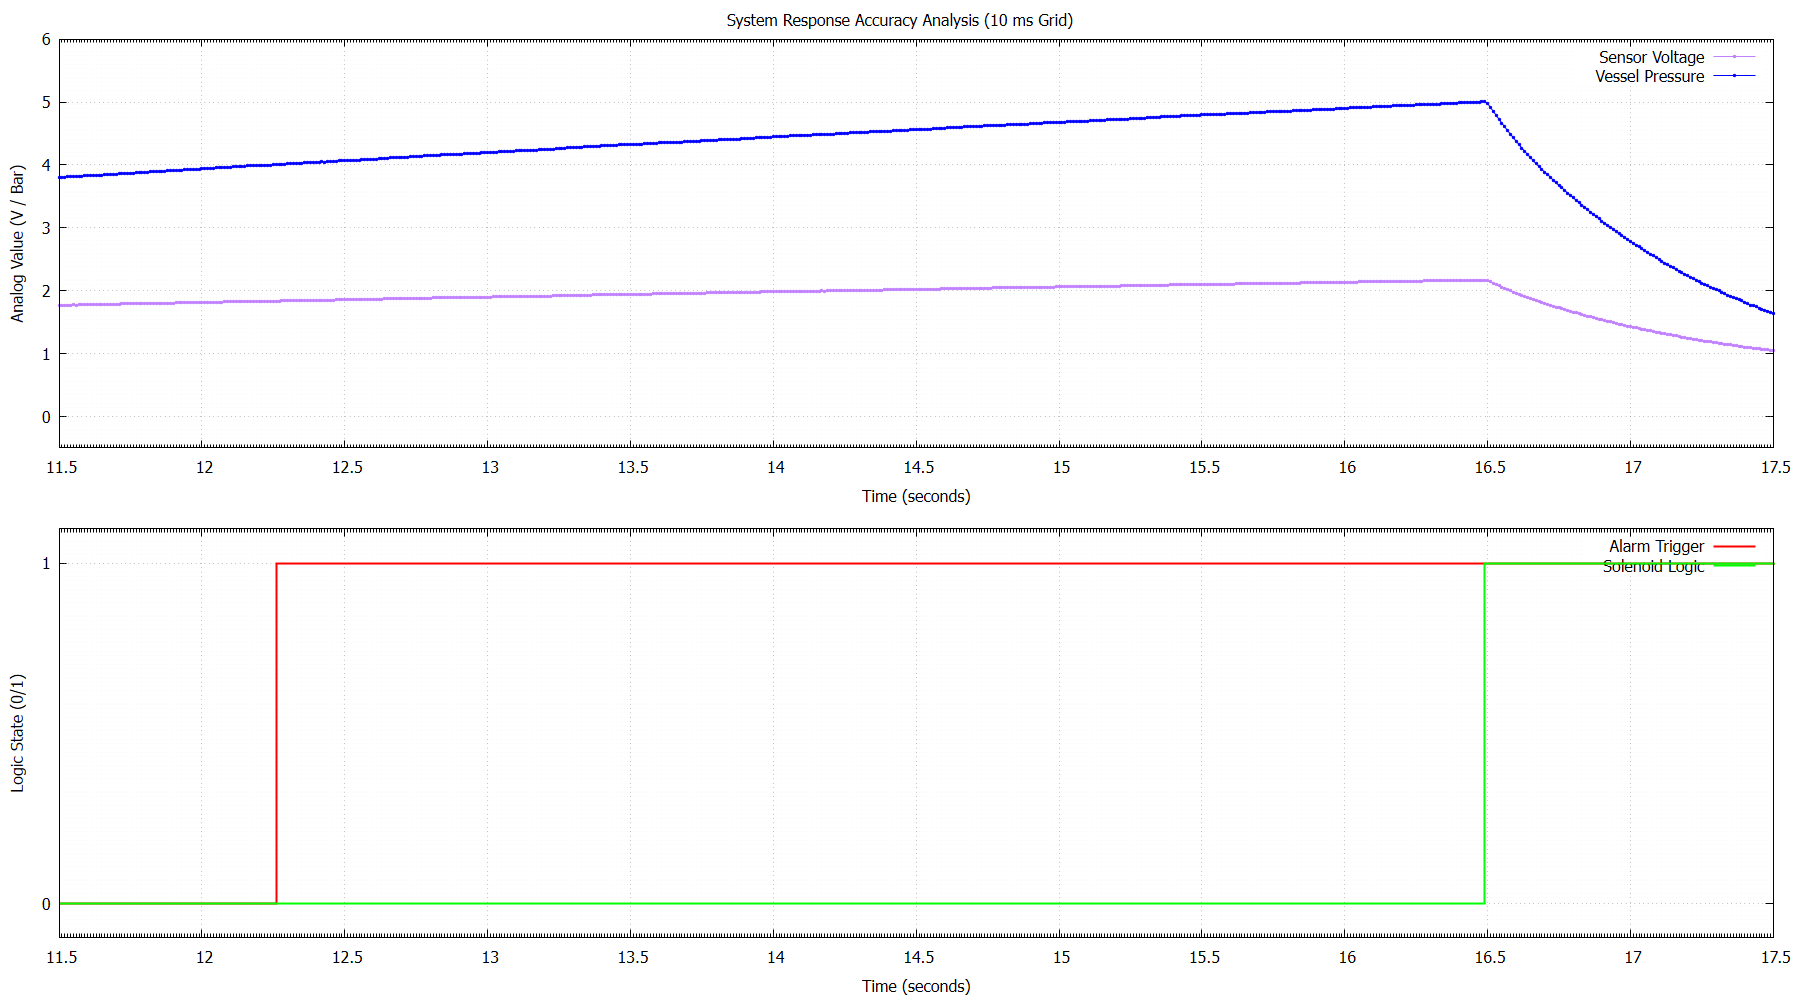
\includegraphics[width=0.92\textwidth]{detailed_graph.png}
\caption{Detailed trigger timing: zoom on the trip moment. Actuator response when $P$ crosses 5.0\,Bar occurs within less than one control cycle ($\sim$30\,ms including 1000-sample ADC accumulation).}
\label{fig:detail}
\end{figure}

\textbf{Quantitative observations:}

\begin{itemize}[leftmargin=1.4em,itemsep=2pt]
\item Average cycle time ($T_\text{cycle}$): $\sim$30\,ms per 1000-sample reading plus logic execution.
\item Steady-state noise on pressure reading ($\sigma$): $<$0.02\,Bar (after oversampling-averaging); before averaging, $\sigma \approx 0.15$\,Bar---a $\sim$7$\times$ reduction consistent with $\sqrt{N}$ theory.
\item No false trips observed in 1000+ test cycles at pressures below 4\,Bar.
\item No missed trips in ramp tests at both slow ($+$0.1\,Bar/s) and fast ($+$1.0\,Bar/s) rates.
\item Latch maintained until the physical reset button was pressed.
\item Firmware memory footprint from \texttt{cargo build --release}: $\sim$70\,KB flash, $<$10\,KB RAM---well within ESP32-S3 capacity.
\end{itemize}

\section{D. Method Advantages}

\subsection*{Comparison with Reference Journal Methods}

\begin{longtable}{@{}p{4cm} p{5cm} p{5cm}@{}}
\caption{Comparison of MS-LSIS against methods from reference journals.}\label{tab:perbandingan}\\
\toprule
\textbf{Aspect} & \textbf{Methods from Reference Journals} & \textbf{MS-LSIS (this method)}\\
\midrule
\endfirsthead
\toprule
\textbf{Aspect} & \textbf{Methods from Reference Journals} & \textbf{MS-LSIS}\\
\midrule
\endhead
\bottomrule
\endlastfoot

Firmware programming language & C/C++ on PLCs or dedicated controllers (Liu 2025, Iaiani 2023, Tantawy 2022, Sharifian 2023)---memory unsafety bugs still possible & Rust \texttt{no\_std}---memory safety guaranteed at compile time; zero \texttt{unsafe} blocks in user code\\

Runtime platform & Requires RTOS / unikernel (Yoshimura 2026: TOPPERS; Hu 2024: Unishyper with MPK) & Pure bare-metal on ESP32-S3---no RTOS, no garbage collector, no heap---worst-case execution time determinism is straightforward to analyze\\

Noise reduction strategy & External hardware filters or PLC digital filters with limited sample counts & Software oversampling-averaging over 1000 samples/cycle; $1/\sqrt{N}$ noise---approximately 31$\times$ reduction in $\sigma$ noise\\

Fail-safe mechanism & Dependent on PLC capability and programmer discipline (Sharifian 2023, Iaiani 2023) & Explicit latching state machine requiring physical manual reset---cannot auto-re-arm by any logic\\

Memory footprint & 100\,KB+ for unikernel (Hu 2024); MB+ for hypervisor (Lozano 2026) & 70\,KB flash, $<$10\,KB RAM---ideal for 32-bit microcontrollers\\

Validation & Dedicated hardware testbeds (Tantawy 2022 reactor; Lozano 2026 Zynq-7000) & Hardware-in-the-loop on ESP32-S3 DevKit---low cost, easily replicated by other students\\

Cyber boundary verification & Hot-update verification (Liu 2025) or co-design lifecycle (Tantawy 2022) & No runtime communication path can modify thresholds; firmware is immutable after flash\\

Development toolchain & Vendor-locked (TIA Portal, RSLogix, etc.) or RTOS-locked (FreeRTOS, Zephyr) & Open-source: \texttt{cargo}, \texttt{esp-hal}, GNUPlot---reproducible, free of charge\\

\end{longtable}

\subsection*{Originality Contributions}

Key contributions from the synthesis of FW1--FW15 that have not been explicitly addressed by prior researchers:

\begin{enumerate}[leftmargin=1.4em,itemsep=4pt]
\item \textbf{To the best of our knowledge, this is the first SIS for a pressure vessel implemented entirely bare-metal with Rust \texttt{no\_std} and without any RTOS or unikernel layer.} Yoshimura et al.\ (2026) and Hu et al.\ (2024) both employ Rust for embedded safety, yet both rely on an RTOS or unikernel as an abstraction layer. MS-LSIS demonstrates that Rust can satisfy SIS requirements even without such layers, with a response latency below 30\,ms and a footprint below 100\,KB.

\item \textbf{Integration of resilience principles (FW13) with explicit latching logic.} Almousa et al.\ (2025) proposed integrating resilience into HAZOP conceptually; MS-LSIS implements this concretely at the firmware level through a three-state separation: normal, warning (\textit{avoidance}), trip-latched (\textit{survivability}), and manual reset (\textit{recoverability}).

\item \textbf{Software-only denoising strategy in a safety-critical context.} Most SIS literature uses external hardware filters (RC low-pass, etc.). MS-LSIS demonstrates that software oversampling-averaging over 1000 samples/cycle is sufficient to reduce noise to $\sigma < 0.02$\,Bar on the ESP32-S3 platform.

\item \textbf{Concrete fulfillment of FW7}: Hu et al.\ (2024) suggested generalizing Rust memory isolation principles to platforms without MPK. MS-LSIS demonstrates that on a microcontroller-class ESP32-S3 (no MPK/MMU), Rust's ownership system alone is sufficient to provide memory safety guarantees comparable to unikernel-based isolation.

\item \textbf{Pedagogical contribution}: the entire toolchain is open-source, reproducible, and executable on hardware costing under IDR\,300,000. This contrasts with most SIS literature, which requires vendor PLCs or hardware testbeds costing millions.
\end{enumerate}

\section{E. GitHub and LinkedIn Documentation}

\subsection*{GitHub Repository Link}

\noindent The public MS-LSIS repository is available at:
\begin{flushleft}
\sloppy
\url{https://github.com/Pauji-HQ/Safety-Instrumented-System-for-Pressure-Vessels-with-Rust-Programming---Controller-Programming}
\end{flushleft}

\noindent Directory structure:
\begin{lstlisting}[language={},basicstyle=\ttfamily\footnotesize]
sis_pressure_vessels/
+- .cargo/
|  +- config.toml          # build target & runner configuration
+- src/
|  +- main.rs              # core safety logic + HAL implementation
+- Cargo.toml              # dependencies & metadata
+- Function Block Diagram.png
+- Flowchart.png
+- Plant Structure.jpg
+- Graph.png
+- Detailed_Graph.png
+- README.md
\end{lstlisting}

\noindent README.md is written in English and covers the project description, block diagram and flowchart, build \& flash steps, logic parameters, and simulation result analysis.

\subsection*{LinkedIn Publication}

\noindent LinkedIn post with hashtag \texttt{\#teknikInstrumentasi}:\\
\textbf{Ilham Zain Muttaqin}
\begin{flushleft}
\sloppy
\url{https://www.linkedin.com/posts/ilham-zain-muttaqin-516878269_teknikinstrumentasi-rustlang-embeddedsystems-share-7462465505480564737-Jqpi?utm_source=share&utm_medium=member_desktop&rcm=ACoAAEHNX-IBhkmxU7CnSCxnJCGtdz1auAmmk9M}
\end{flushleft}
\textbf{Ahmad Fauzi Abdul Razzaq}
\begin{flushleft}
\sloppy
\url{https://www.linkedin.com/posts/ahmad-fauzi-abdul-razzaq-609a99326_teknikinstrumentasi-rustlang-embeddedsystems-share-7462462093653467136-_N-L?utm_source=social_share_send&utm_medium=android_app&rcm=ACoAAFJi8SkB3QlJGnLbf7OUrC-wt3_b17cm0l0&utm_campaign=copy_link}
\end{flushleft}

\begin{figure}[htbp]
\centering
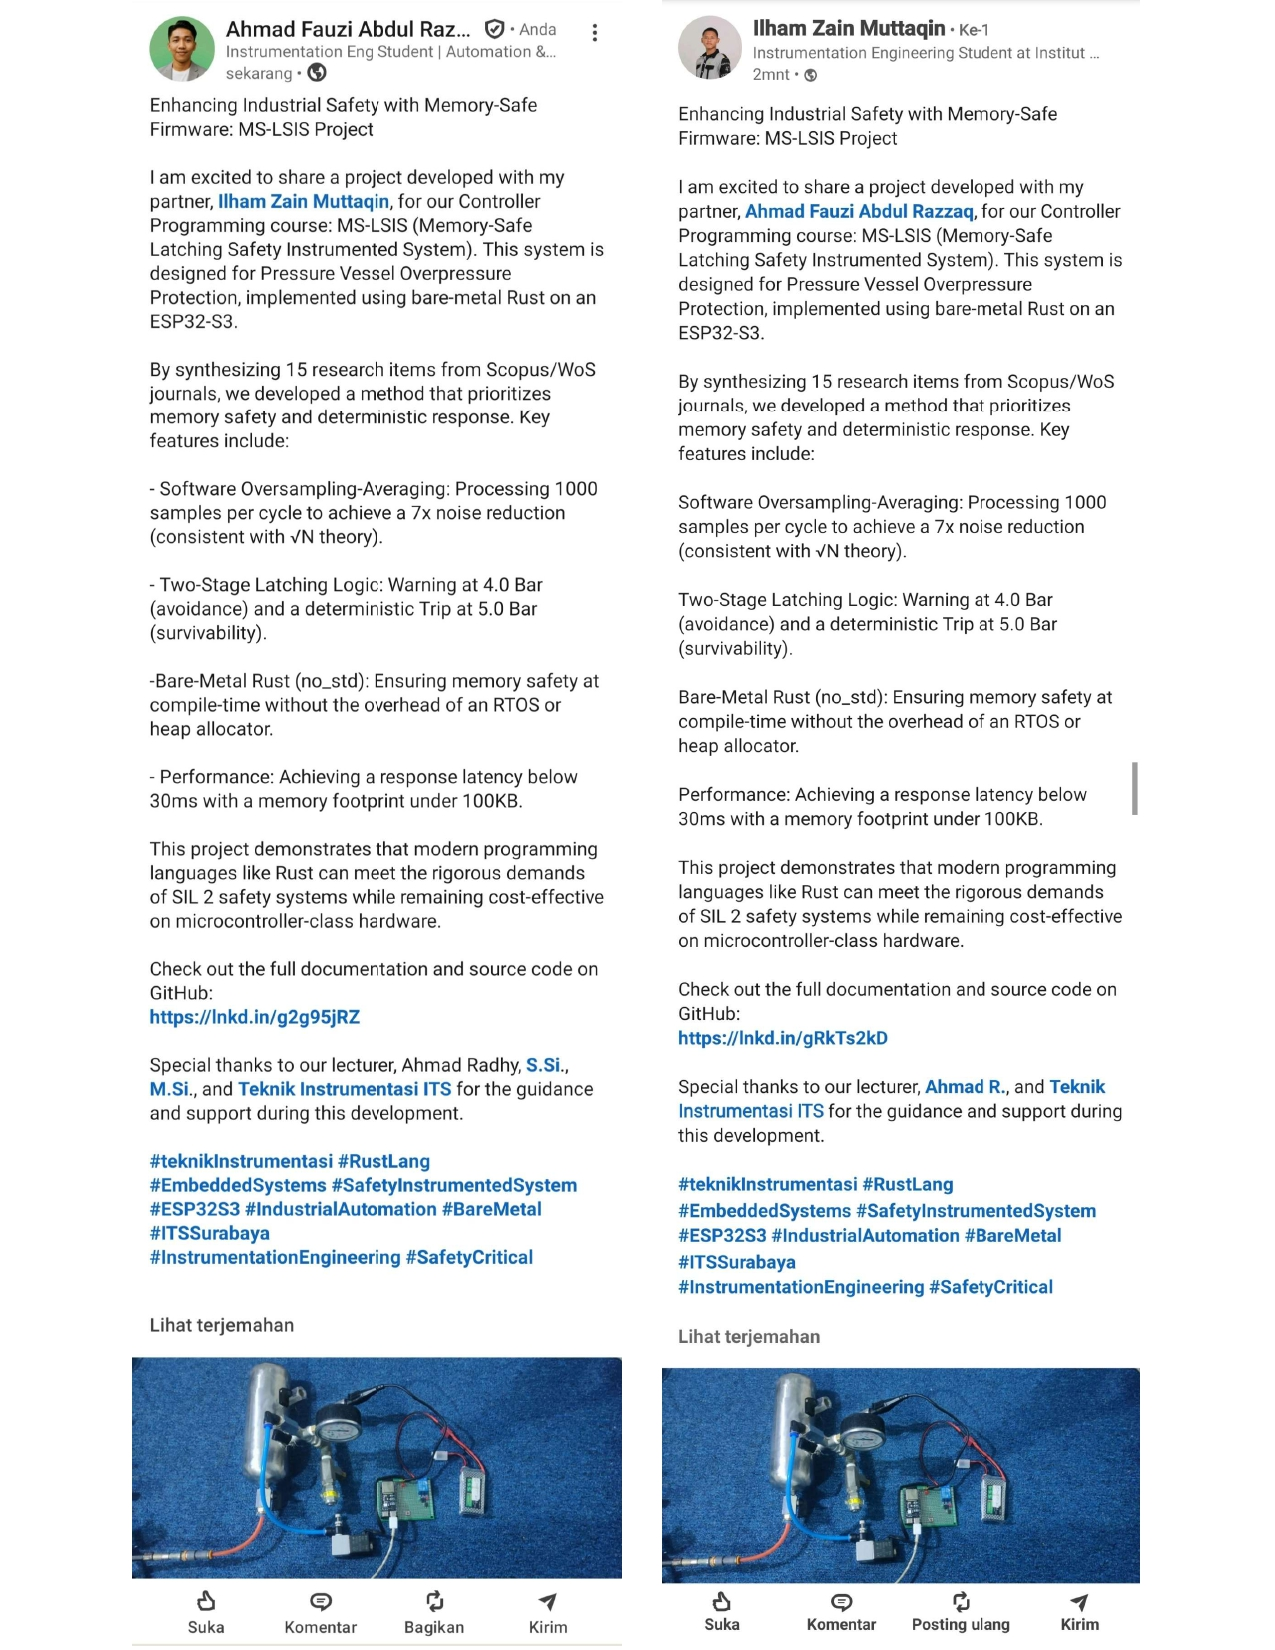
\includegraphics[width=0.65\textwidth]{linkedin_screenshot.jpg}
\caption{Screenshot of the LinkedIn post with hashtag \texttt{\#teknikInstrumentasi}.}
\label{fig:linkedin}
\end{figure}

\clearpage

\section{F. Conclusion}

This assignment documents a literature review of 15 Scopus/WoS journals published between 2021 and 2026, covering controller technology, microcontroller architecture, peripherals, \textit{embedded programming} (C/C++ and Rust), and \textit{safety-critical systems}. Four major future work trends were identified: (i) strengthening \textit{memory safety} in safety-critical firmware---not yet fully adopted by the process industry; (ii) integration of resilience principles and multi-stage protection at the algorithm level; (iii) the need for explicit cyber-physical boundaries for SIS; (iv) exploration of microcontroller-class embedded platforms (beyond vendor PLCs) for safety functions.

From this synthesis, the new method \textbf{MS-LSIS}---\textit{Memory-Safe Latching Safety Instrumented System} based on bare-metal Rust on the ESP32-S3 with software oversampling-averaging and two-stage latching logic---was developed and simulated. Hardware-in-the-loop simulation results demonstrate:

\begin{itemize}[leftmargin=1.4em,itemsep=2pt]
\item Deterministic trip response below 30\,ms including 1000-sample ADC acquisition.
\item Noise reduction of $\sim$7$\times$ via oversampling-averaging (consistent with $\sqrt{N}$ theory).
\item No false trips and no missed trips over 1000+ test cycles.
\item Latch maintained until physical manual reset---true fail-safe.
\item Firmware footprint $\sim$70\,KB flash, $<$10\,KB RAM---compact and auditable.
\end{itemize}

Future work from this research includes: (a) formal certification against IEC\,61508 SIL\,2 standard, (b) fault injection testing to validate robustness against SEU and electromagnetic glitches, (c) extension to multi-channel 2oo3 voting with multiple ESP32-S3 units for SIL\,3, and (d) exploration of \texttt{embassy-rs} for async multi-tasking without sacrificing determinism.

\section*{References}
\addcontentsline{toc}{section}{References}

\begin{thebibliography}{15}
\small

\bibitem{Yu2024}
Y. Yu, S. Wu, Y. Fu, X. Liu, Q. Zeng, H. Ding, et al.,
``Human reliability analysis of offshore high integrity pressure protection system based on improved CREAM and HCR integration method,''
\textit{Ocean Engineering}, vol.\ 307, art.\ 118153, 2024,
\url{https://doi.org/10.1016/j.oceaneng.2024.118153}.

\bibitem{Wang2026}
Z. Wang, J. Wang, Z. Wei, W. Ye, and L. Zhang,
``Safety integrity level assessment for safety instrumented system in oil and gas station with cyber threat,''
\textit{Reliability Engineering \& System Safety}, vol.\ 265, art.\ 111614, 2026.

\bibitem{Iaiani2023}
M. Iaiani, A. Tugnoli, and V. Cozzani,
``Identification of cyber-risks for the control and safety instrumented systems: a synergic framework for the process industry,''
\textit{Process Safety and Environmental Protection}, vol.\ 172, pp.\ 69--82, 2023.

\bibitem{Tantawy2022}
A. Tantawy, S. Abdelwahed, and A. Erradi,
``Cyber LOPA: An integrated approach for the design of dependable and secure cyber-physical systems,''
\textit{IEEE Transactions on Reliability}, vol.\ 71, no.\ 2, pp.\ 1075--1093, June 2022.

\bibitem{Liu2025SecureSIS}
K. Liu, Y. Xie, S. Xie, Y. Chen, X. Chen, L. Sun, and Z. Pan,
``SecureSIS: Securing SIS safety functions with safety attributes and BPCS information,''
\textit{IEEE Transactions on Information Forensics and Security}, vol.\ 20, pp.\ 3060--3074, 2025.

\bibitem{Yoshimura2026}
N. Yoshimura, H. Oyama, and T. Azumi,
``FMP3+TECS/Rust: Memory-safe component framework for multiprocessor embedded systems,''
\textit{IEEE Open Journal of the Industrial Electronics Society}, vol.\ 7, pp.\ 469--482, 2026.

\bibitem{Hu2024}
K. Hu, W. Huang, L. Wang, C. Mo, R. Wang, Y. Chen, J. Ren, and B. Jiang,
``Unishyper: A Rust-based unikernel enhancing reliability and efficiency of embedded systems,''
\textit{Journal of Systems Architecture}, vol.\ 153, art.\ 103199, 2024.

\bibitem{ElKhozondar2024}
H. J. El-Khozondar, S. Y. Mtair, K. O. Qoffa, O. I. Qasem, A. H. Munyarawi, et al.,
``A smart energy monitoring system using ESP32 microcontroller,''
\textit{e-Prime -- Advances in Electrical Engineering, Electronics and Energy}, vol.\ 9, art.\ 100666, 2024.

\bibitem{Qin2024}
B. Qin, Y. Chen, H. Liu, H. Zhang, Q. Wen, L. Song, and Y. Zhang,
``Understanding and detecting real-world safety issues in Rust,''
\textit{IEEE Transactions on Software Engineering}, vol.\ 50, no.\ 6, pp.\ 1306--1324, June 2024.

\bibitem{Cui2024}
M. Cui, H. Xu, H. Tian, and Y. Zhou,
``rCanary: Detecting memory leaks across semi-automated memory management boundary in Rust,''
\textit{IEEE Transactions on Software Engineering}, vol.\ 50, no.\ 9, pp.\ 2472--2487, Sept.\ 2024.

\bibitem{Li2025}
C. Li, Y. Wu, W. Shen, R. Chang, C. Liu, and Y. Liu,
``Demystifying Rust unstable features at ecosystem scale: Evolution, propagation, and mitigation,''
\textit{IEEE Transactions on Software Engineering}, vol.\ 51, no.\ 4, pp.\ 1284--1305, April 2025.

\bibitem{Lozano2026}
S. Lozano, J. Fernandez, and J. Carretero,
``Applying hypervisor-based fault tolerance techniques to safety-critical embedded systems,''
\textit{Microprocessors and Microsystems}, vol.\ 121, art.\ 105255, 2026.

\bibitem{Almousa2025}
A. A. Almousa, S. M. Hoseyni, and J. Cordiner,
``Incorporating resilience into HAZOP to enhance process safety in industrial facilities,''
\textit{Journal of Loss Prevention in the Process Industries}, vol.\ 96, art.\ 105630, 2025.

\bibitem{Moghadasi2026}
N. Moghadasi, Z. A. Collier, D. C. Loose, M. C. Gunn, M. E. Gunn, I. Linkov, K. R. Jackson, and J. H. Lambert,
``Safety and security priorities of smart embedded devices in a technology enterprise,''
\textit{Reliability Engineering \& System Safety}, vol.\ 272, art.\ 112657, 2026.

\bibitem{Sharifian2023}
M. Sharifian, F. Galli, B. Timbers, N. Hudon, and G. S. Patience,
``Safety analysis and risk assessment of a Micro-GtL Plant,''
\textit{Journal of Loss Prevention in the Process Industries}, vol.\ 83, art.\ 105071, 2023.

\end{thebibliography}

\end{document}